% Salia sio .tex failo turi buti Mokinio_originalas.pdf.
% Mokinio sprendimai rodomi kaip originalaus PDF iskarpos, ne transkripcija.
\documentclass[11pt,a4paper]{article}
\usepackage[T1]{fontenc}
\usepackage[utf8]{inputenc}
\usepackage[lithuanian]{babel}
\usepackage{lmodern}
\usepackage{amsmath,amssymb}
\usepackage[a4paper,margin=1.8cm]{geometry}
\usepackage{enumitem}
\usepackage{xcolor}
\usepackage{fancyhdr}
\usepackage{microtype}
\usepackage{graphicx}
\definecolor{ink}{HTML}{203C50}
\setlength{\parindent}{0pt}
\setlength{\parskip}{4pt}
\setlist[itemize]{leftmargin=*,itemsep=3pt,topsep=3pt}
\setlength{\abovedisplayskip}{7pt}
\setlength{\belowdisplayskip}{7pt}
\pagestyle{fancy}
\fancyhf{}
\fancyhead[L]{\small Kvadratinių lygčių uždaviniai}
\fancyhead[R]{\small }
\fancyfoot[C]{\thepage}
\setlength{\headheight}{14pt}
\newcommand{\uzd}[2]{\begin{center}{\Large\bfseries\color{ink}#1 uždavinys}\end{center}\textbf{Sąlyga.} #2\par}
\newcommand{\dalis}[1]{\par\vspace{5pt}{\bfseries\color{ink}#1}\par}
\newcommand{\past}{\dalis{2. Pastabos mokiniui}}
\newcommand{\tais}{\dalis{3. Tvarkingas pataisytas sprendimas}}
\newcommand{\qed}{\hfill$\square$}
\begin{document}
\begin{center}
{\LARGE\bfseries Kvadratinių lygčių uždaviniai}\par
{\normalsize Pastabos ir patarimai}
\end{center}

\uzd{1}{Įrodykite, kad $x^2+(a+b)x+ab-c^2=0$ turi bent vieną realųjį sprendinį visiems $a,b,c\in\mathbb R$. Kada sprendinys vienintelis?}
\begin{center}
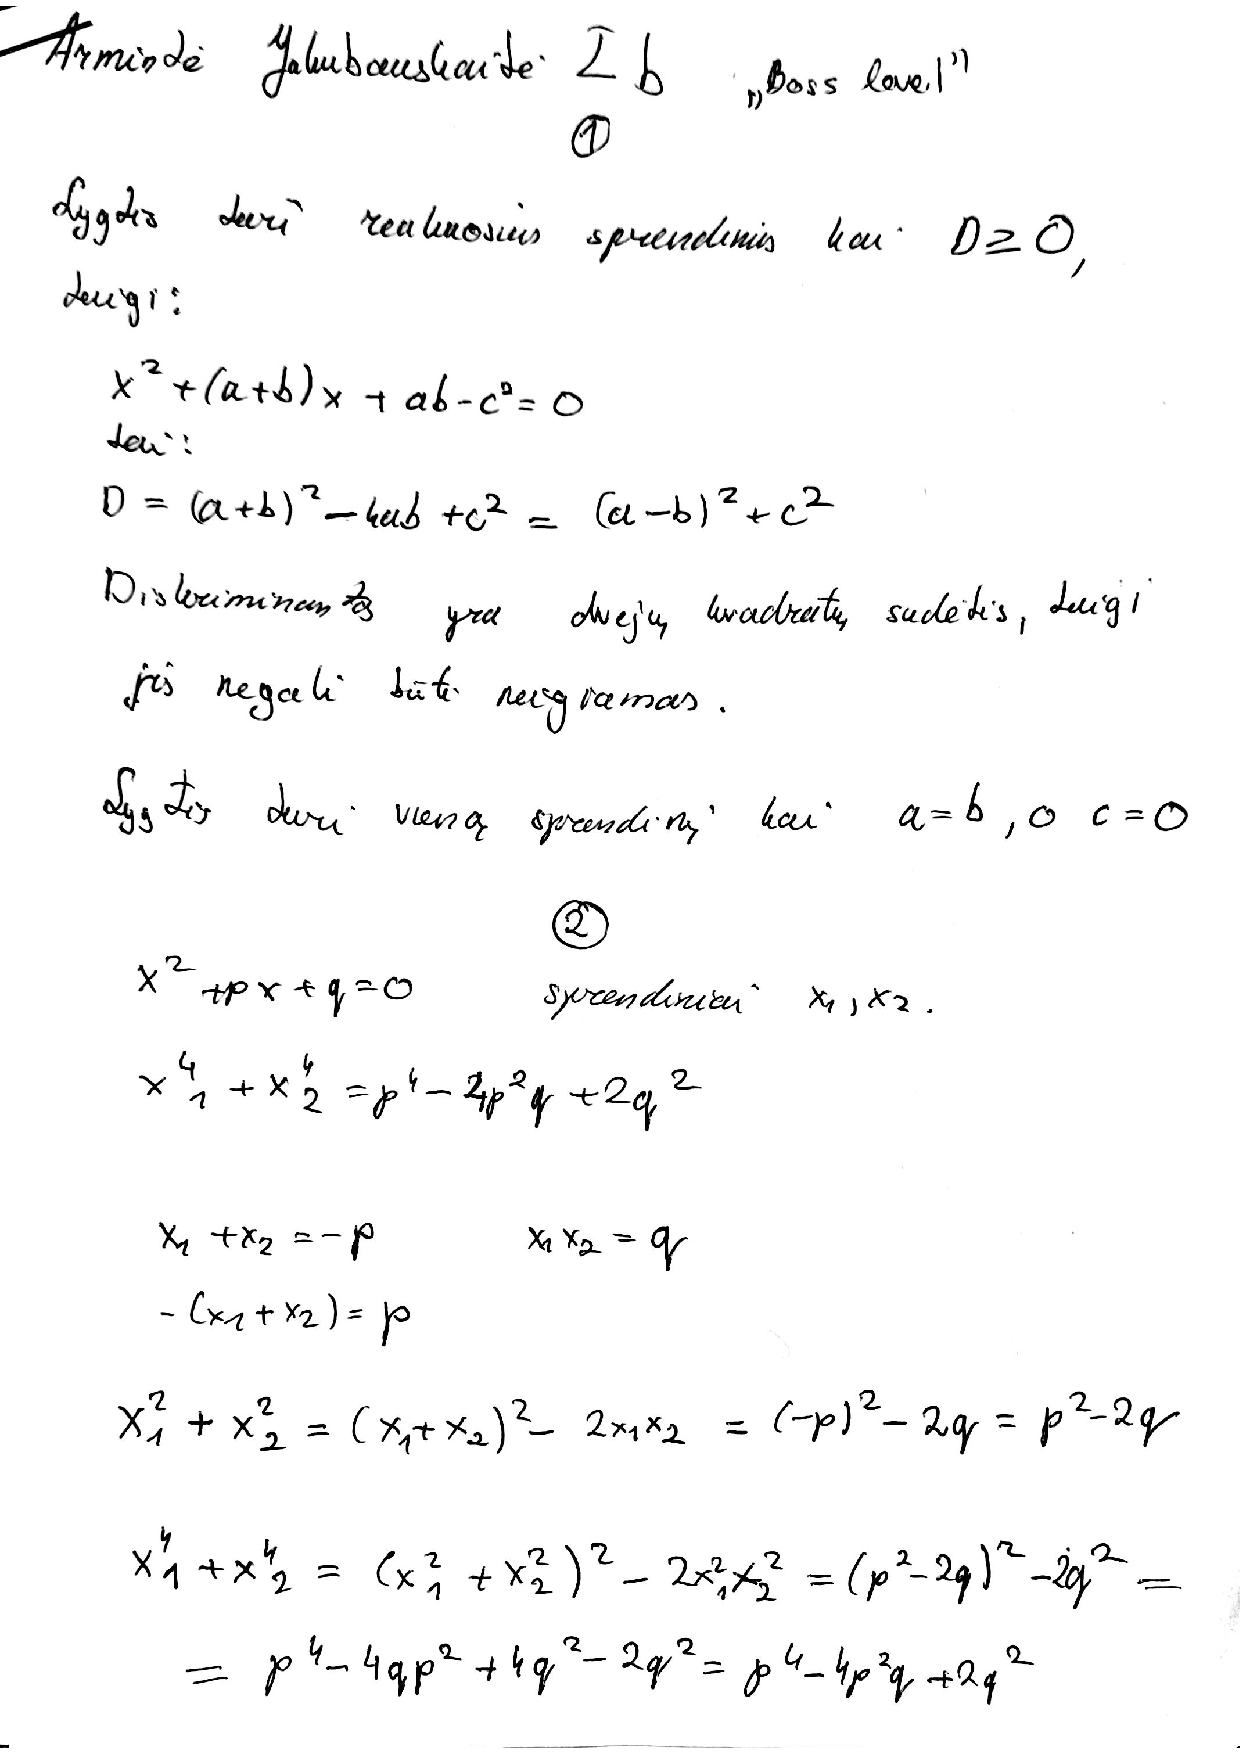
\includegraphics[page=1,trim={11.694 421.000 10.291 51.456},clip,width=\linewidth,height=.68\textheight,keepaspectratio]{Mokinio_originalas.pdf}\par
\end{center}
{\large\bfseries\color{ink}Pastabos ir pataisytas įrodymas}\par
\past
\begin{itemize}
\item Diskriminante praleistas daugiklis $4$ prie $c^2$: $-4(ab-c^2)=-4ab+4c^2$. Todėl turi būti $D=(a-b)^2+4c^2$, o ne $(a-b)^2+c^2$. Tikiu, kad žioplumo klaida :) bet visgi apmaudu jei olimpiadoje tokią palikti.
\item Vienintelio sprendinio sąlygą susiek su $D=0$: paaiškink, kad neneigiamų dėmenų suma lygi nuliui tik tada, kai abu dėmenys nuliai. Vienintelio sprendinio sąlyga $a=b$, $c=0$ po skaičiavimo pataisos nesikeičia.
\end{itemize}
\tais
Lygties diskriminantas yra
\[
D=(a+b)^2-4(ab-c^2)
=a^2-2ab+b^2+4c^2=(a-b)^2+4c^2.
\]
Kadangi realiųjų skaičių kvadratai neneigiami, $D\ge0$. Kvadratinės lygties vyriausiasis koeficientas lygus $1\ne0$, todėl ji turi bent vieną realųjį sprendinį.

Lygtis turi lygiai vieną realųjį sprendinį tada ir tik tada, kai $D=0$. Neneigiamų dėmenų suma lygi nuliui tada, kai abu dėmenys lygūs nuliui. Todėl
\[
D=0\iff a-b=0\ \text{ir}\ c=0
\iff a=b\ \text{ir}\ c=0.
\]
Taigi vienintelis sprendinys yra būtent tada, kai $a=b$ ir $c=0$; tuo atveju lygtis yra $(x+a)^2=0$, o jos sprendinys $x=-a$.\qed

\uzd{2}{Lygties $x^2+px+q=0$ sprendiniai yra $x_1,x_2$. Naudodamiesi Vijeto teorema įrodykite $x_1^4+x_2^4=p^4-4p^2q+2q^2$.}
\begin{center}
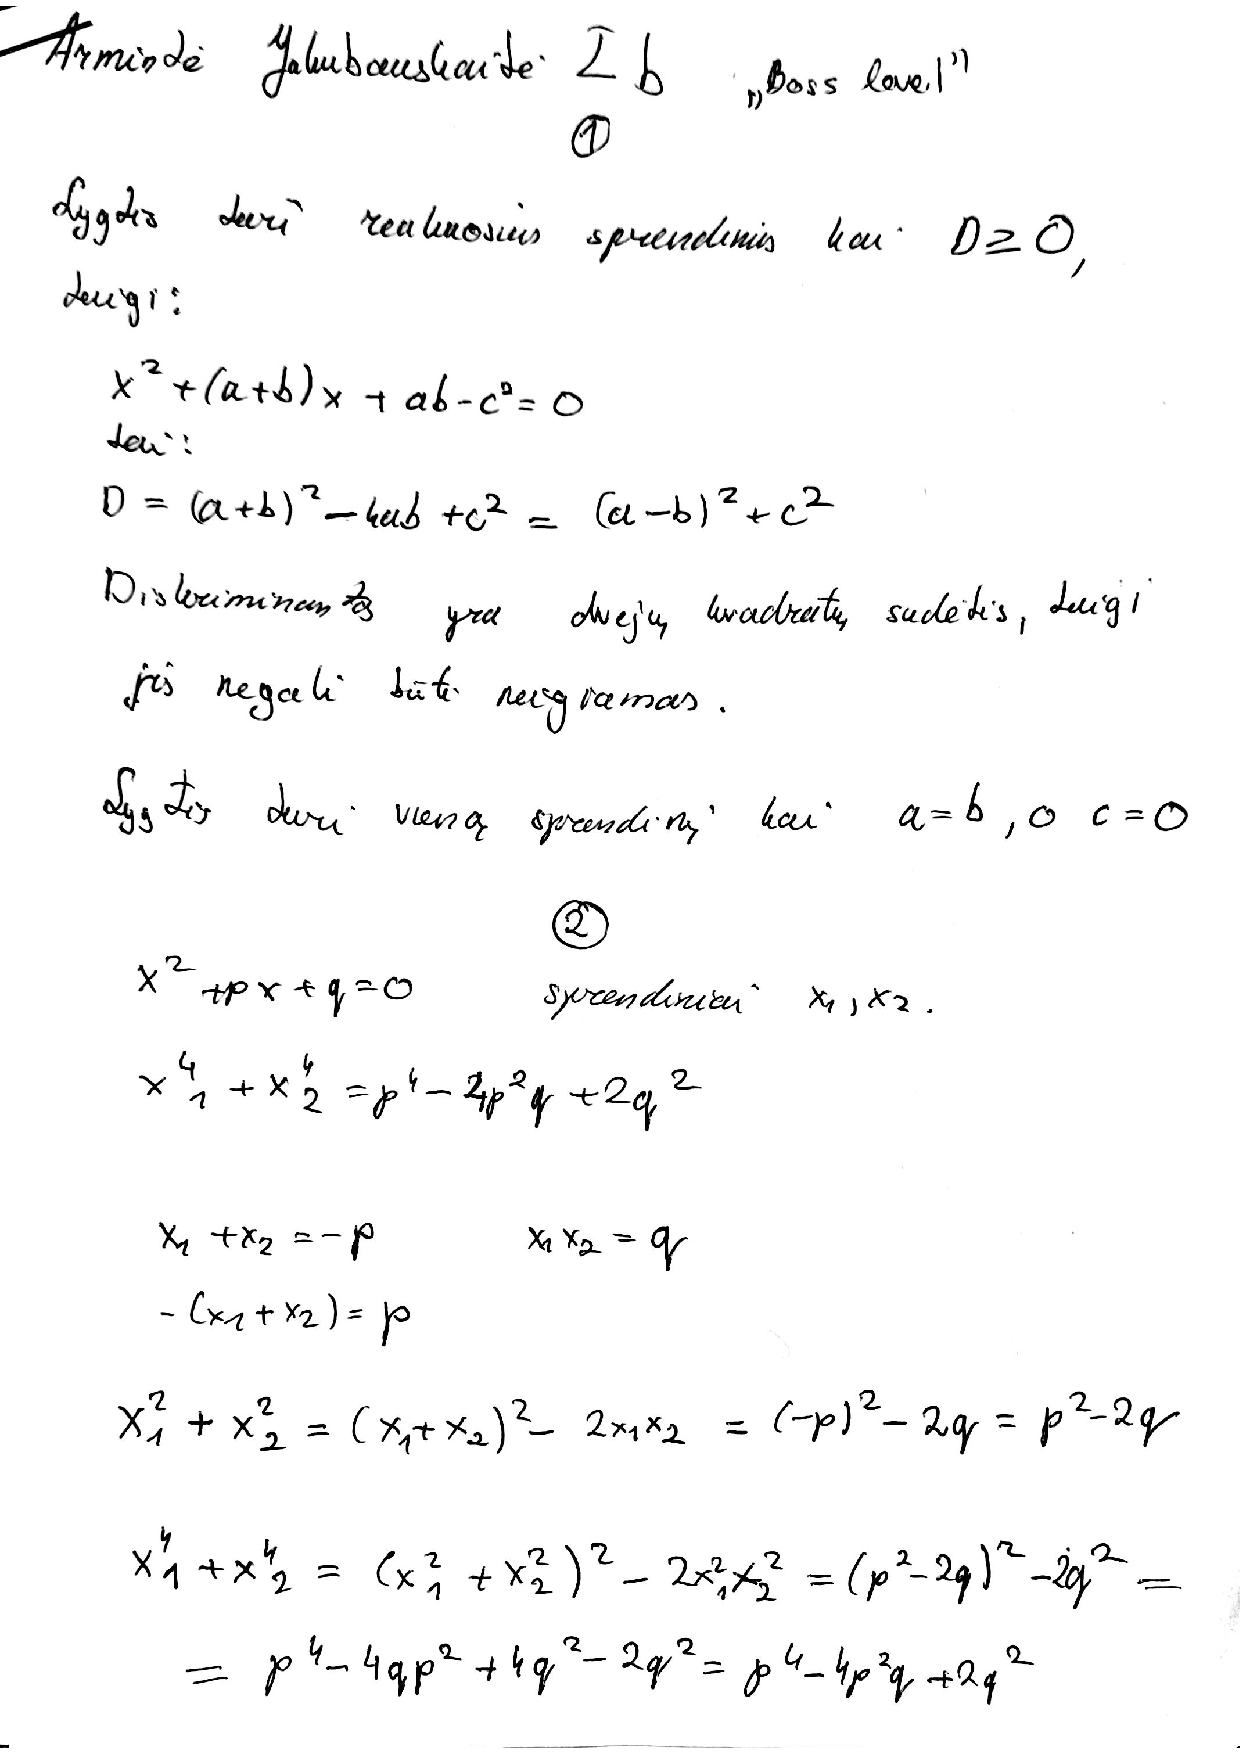
\includegraphics[page=1,trim={11.694 4.678 10.291 428.017},clip,width=\linewidth,height=.76\textheight,keepaspectratio]{Mokinio_originalas.pdf}\par
\end{center}
{\large\bfseries\color{ink}Pastabos ir pataisytas įrodymas}\par
\past
\begin{itemize}
\item Prieš šaknų sumos ir sandaugos lygybes įrašyk „Pagal Vijeto teoremą“. Tai aiškiai nurodys iš kur tos lygybės; atskirų komentarų prie kiekvieno algebrinio veiksmo nereikia.
\end{itemize}
\tais
Pagal Vijeto teoremą
\[
x_1+x_2=-p,\qquad x_1x_2=q.
\]
Naudodamiesi sumos kvadrato tapatybe, gauname
\[
x_1^2+x_2^2=(x_1+x_2)^2-2x_1x_2=p^2-2q.
\]
Todėl
\begin{align*}
x_1^4+x_2^4
&=(x_1^2+x_2^2)^2-2x_1^2x_2^2\\
&=(p^2-2q)^2-2q^2\\
&=p^4-4p^2q+4q^2-2q^2\\
&=p^4-4p^2q+2q^2.
\end{align*}
Reikiama tapatybė įrodyta.\qed

\uzd{3}{Lygtys $x^2+px+q=0$ ir $x^2+qx+p=0$, kur $p\ne q$, turi bendrą realųjį sprendinį. Įrodykite, kad $p+q+1=0$.}
\begin{center}
\includegraphics[page=2,trim={7.017 70.167 7.952 7.017},clip,width=\linewidth,height=.76\textheight,keepaspectratio]{Mokinio_originalas.pdf}\par
\end{center}
{\large\bfseries\color{ink}Pastabos ir pataisytas įrodymas}\par
\past
\begin{itemize}
\item Pradžioje apibrėžk $x$: „Tegu $x$ -- bendras abiejų lygčių realusis sprendinys.“ Tada aišku, kodėl abi lygybės galioja tam pačiam skaičiui. Nors geriau būtų koks $x_0$ ir pan. 
\item Išvadą pakanka gauti įstačius $x=1$ į vieną lygtį. Įstatymas į antrąją nėra klaida, bet kartoja tą patį rezultatą.
\end{itemize}
\tais
Tegu $x_0$ yra bendras abiejų lygčių realusis sprendinys. Tuomet
\[
x_0^2+px_0+q=0,\qquad x_0^2+qx_0+p=0.
\]
Atėmę antrąją lygybę iš pirmosios, gauname
\[
(x_0^2+px_0+q)-(x_0^2+qx_0+p)=0.
\]
Vadinasi,
\[
(p-q)x_0+q-p=0,
\qquad (p-q)(x_0-1)=0.
\]
Kadangi $p\ne q$, turime $p-q\ne0$. Todėl $x_0-1=0$, t.\,y. $x_0=1$.

Įstatę $x_0=1$ į pirmąją lygtį, gauname
\[
1+p+q=0.
\]
Taigi $p+q+1=0$, ką ir reikėjo įrodyti.\qed
\newpage
\uzd{4}{Lygtis $ax^2+bx+c=0$, kur $a>0$, neturi realiųjų sprendinių. Įrodykite, kad $a+b+c>0$.}
\begin{center}
\includegraphics[page=3,trim={7.017 201.144 7.952 9.356},clip,width=\linewidth,height=.76\textheight,keepaspectratio]{Mokinio_originalas.pdf}\par
\end{center}
{\large\bfseries\color{ink}Pastabos ir pataisytas įrodymas}\par
\past
\begin{itemize}
\item Iš $a+c\le-b$ negalima besąlygiškai pereiti prie $(a+c)^2\le b^2$: kėlimas kvadratu išsaugo nelygybę, kai abi pusės neneigiamos. Pavyzdžiui, $-3\le2$, tačiau $9\nleq4$.
\item Prieš šį žingsnį iš $D<0$ ir $a>0$ išvesk $c>0$. Tada $a+c>0$, o pagal prieštaros prielaidą $-b\ge a+c>0$; kėlimas kvadratu bus teisėtas.
\item Prieštarą įvardyk tiksliai: gautum neneigiamą kvadratą, mažesnį arba lygų neigiamam diskriminantui.
\end{itemize}
\tais
Kadangi duotoji kvadratinė lygtis neturi realiųjų sprendinių,
\[
D=b^2-4ac<0.
\]
Taigi $4ac>b^2\ge0$. Iš $a>0$ gauname $c>0$, todėl $a+c>0$.

Tarkime priešingai, kad $a+b+c\le0$. Tuomet
\[
a+c\le-b.
\]
Kadangi $a+c>0$, abi šios nelygybės pusės teigiamos. Todėl galime kelti kvadratu ir gauname
\[
(a+c)^2\le(-b)^2=b^2.
\]
Atėmę $4ac$ iš abiejų pusių, turime
\[
(a-c)^2=(a+c)^2-4ac\le b^2-4ac=D<0.
\]
Tai neįmanoma, nes realiojo skaičiaus kvadratas neneigiamas. Prieštaros prielaida klaidinga, todėl $a+b+c>0$.\qed
\newpage
\uzd{5}{Lygčių $x^2+ax+b=0$ ir $x^2+cx+d=0$ koeficientai tenkina $ac=2(b+d)$. Įrodykite, kad bent viena lygtis turi realiųjų sprendinių.}
\begin{center}
\includegraphics[page=4,trim={9.355 350.833 7.952 9.356},clip,width=\linewidth,height=.76\textheight,keepaspectratio]{Mokinio_originalas.pdf}\par
\end{center}
{\large\bfseries\color{ink}Pastabos ir pataisytas įrodymas}\par
\past
\begin{itemize}
\item Reikia įrodyti $D_1\ge0$ \emph{arba} $D_2\ge0$, o ne abu teiginius kartu. Žodis „bent viena“ reiškia, kad pakanka vieno neneigiamo diskriminanto.
\item Iš $D_1+D_2\ge0$ neišplaukia $D_1\ge0$ ir $D_2\ge0$. Pavyzdžiui, $a=c=0$, $b=1$, $d=-1$ tenkina $ac=2(b+d)$, bet $D_1=-4$, $D_2=4$.
\item Užbaik argumentą: jei abu diskriminantai būtų neigiami, jų suma būtų neigiama. Todėl bent vienas neneigiamas ir atitinkama lygtis turi realiųjų sprendinių.
\end{itemize}
\tais
Pažymėkime pirmosios ir antrosios lygčių diskriminantus atitinkamai $D_1$ ir $D_2$. Tuomet
\[
D_1=a^2-4b,\qquad D_2=c^2-4d.
\]
Iš sąlygos $ac=2(b+d)$ gauname $4(b+d)=2ac$. Todėl
\begin{align*}
D_1+D_2
&=a^2+c^2-4(b+d)\\
&=a^2+c^2-2ac\\
&=(a-c)^2\ge0.
\end{align*}
Jeigu abu diskriminantai būtų neigiami, jų suma būtų neigiama. Tai prieštarauja gautai nelygybei. Vadinasi, bent vienas iš skaičių $D_1,D_2$ yra neneigiamas.

Abiejų lygčių vyriausiasis koeficientas lygus $1$. Todėl ta lygtis, kurios diskriminantas neneigiamas, turi bent vieną realųjį sprendinį. Taigi bent viena duotoji lygtis turi realiųjų sprendinių.\qed
\newpage
\uzd{6}{Kvadratinės lygties $ax^2+bx+c=0$, kur $a\ne0$, sprendiniai yra $x_1,x_2$, o $x_2=nx_1$. Įrodykite, kad $nb^2=(n+1)^2ac$.}
\begin{center}
\includegraphics[page=5,trim={11.694 116.944 10.291 7.017},clip,width=\linewidth,height=.76\textheight,keepaspectratio]{Mokinio_originalas.pdf}\par
\end{center}
{\large\bfseries\color{ink}Pastabos ir pataisytas įrodymas}\par
\past
\begin{itemize}
\item Patarimas užrašui: įvardyk Vijeto teoremą prieš naudojamas šaknų sumos ir sandaugos lygybes.
\item Perėjimą, kuriame pakeiti $anx_1^2$ į $c$, geriau pagrįsti sakiniu „Panaudoję $anx_1^2=c$, gauname...“. Taip pažymėtas pakeitimas tampa aiškia įrodymo dalimi.
\end{itemize}
\tais
Pagal Vijeto teoremą
\[
x_1+x_2=-\frac ba,\qquad x_1x_2=\frac ca.
\]
Kadangi $x_2=nx_1$ ir $a\ne0$, šias lygybes galime užrašyti taip:
\[
-ax_1(1+n)=b,\qquad anx_1^2=c.
\]
Pakėlę pirmąją lygybę kvadratu ir padauginę iš $n$, gauname
\[
a^2nx_1^2(1+n)^2=nb^2.
\]
Panaudoję $anx_1^2=c$, kairę pusę pertvarkome:
\[
a^2nx_1^2(1+n)^2=a(anx_1^2)(1+n)^2=ac(1+n)^2.
\]
Vadinasi,
\[
\boxed{nb^2=(n+1)^2ac.}
\]
Reikiama lygybė įrodyta.\qed
\newpage
\uzd{7}{Įrodykite, kad jeigu $a,b,c$ yra nelyginiai sveikieji skaičiai, tai lygtis $ax^2+bx+c=0$ negali turėti sveikojo sprendinio.}
\begin{center}
\includegraphics[page=6,trim={0.000 430.356 0.000 9.356},clip,width=\linewidth,height=.76\textheight,keepaspectratio]{Mokinio_originalas.pdf}\par
\end{center}
{\large\bfseries\color{ink}Pastabos ir pataisytas įrodymas}\par
\past
\begin{itemize}
\item Užrašai $x=N$ ir $x=L$ yra neformalūs: jie atrodo kaip skaičiaus lygybė su simboliu. Rašyk „$x$ nelyginis“ arba „$x$ lyginis“; jei naudoji $N,L$, iš anksto paaiškink, kad tai lyginumo žymenys.
\item Užbaik vienu bendru sakiniu: abiem atvejais $ax^2+bx+c$ nelyginis, todėl negali būti lygus nuliui. Taip aiškiai susiejami abu atvejai ir uždavinio išvada.
\end{itemize}
\tais
Tarkime priešingai, kad egzistuoja sveikasis skaičius $x$, tenkinantis
\[
ax^2+bx+c=0.
\]
Kiekvienas sveikasis skaičius yra lyginis arba nelyginis, todėl nagrinėjame abu atvejus.

\textbf{1 atvejis: $x$ nelyginis.} Tada $x^2$ nelyginis. Kadangi $a,b,c$ nelyginiai, visi trys skaičiai $ax^2$, $bx$, $c$ nelyginiai. Dviejų nelyginių skaičių suma lyginė, o pridėjus trečią nelyginį gaunamas nelyginis skaičius. Taigi $ax^2+bx+c$ nelyginis.

\textbf{2 atvejis: $x$ lyginis.} Tada $x^2$ lyginis, todėl $ax^2$ ir $bx$ lyginiai. Jų suma lyginė, o pridėjus nelyginį $c$ gaunamas nelyginis skaičius. Taigi ir šiuo atveju $ax^2+bx+c$ nelyginis.

Abiem atvejais $ax^2+bx+c$ nelyginis ir todėl negali būti lygus nuliui, nes nulis lyginis. Gavome prieštarą. Vadinasi, lygtis neturi sveikojo sprendinio.\qed
\newpage
\uzd{8}{Jeigu $p,q\in\mathbb Z$, o lygties $x^2+px+q=0$ diskriminantas yra sveikojo skaičiaus kvadratas, įrodykite, kad visi sprendiniai sveikieji.}
\begin{center}
\includegraphics[page=6,trim={0.000 0.000 0.000 421.000},clip,width=\linewidth,height=.76\textheight,keepaspectratio]{Mokinio_originalas.pdf}\par
\end{center}
{\large\bfseries\color{ink}Pastabos ir pataisytas įrodymas}\par
\past
\begin{itemize}
\item Teiginys, kad $p$ ir $q$ turi būti vienodo lyginumo, klaidingas. Pavyzdžiui, $p=3$, $q=2$: $D=1$ yra sveikojo skaičiaus kvadratas, tačiau $p$ nelyginis, o $q$ lyginis. Reikia palyginti $p$ ir $k$, ne $p$ ir $q$.
\item Sveikojo skaičiaus kvadratas gali būti nulis, todėl iš sąlygos gaunama $D\ge0$, ne būtinai $D>0$. Pavyzdžiui, $p=2$, $q=1$ duoda $D=0$.
\item Iš lygybės $(p-k)(p+k)=4q$ parodyk, kad priešingo $p$ ir $k$ lyginumo atveju abu dauginamieji būtų nelyginiai, o jų sandauga negalėtų būti lygi lyginiam skaičiui $4q$. Šis argumentas apima abu priešingo lyginumo atvejus.
\item Po šio palyginimo dar parašyk, kodėl abu skaičiai $(-p+k)/2$ ir $(-p-k)/2$ sveikieji. Pasirink $k\ge0$, kad $\sqrt D=k$.
\end{itemize}
\textit{Skeno apačioje paskutinė eilutė yra ties lapo riba; pastabos grindžiamos perskaitoma sprendimo dalimi.}
\tais
Pagal sąlygą egzistuoja sveikasis $m$, kuriam $D=m^2$. Pasirinkime $k=|m|\in\mathbb Z$, $k\ge0$. Tuomet
\[
p^2-4q=k^2,\qquad p^2-k^2=4q,
\]
todėl
\[
(p-k)(p+k)=4q.
\]
Įrodysime, kad $p$ ir $k$ vienodo lyginumo. Tarkime priešingai, kad vienas iš jų lyginis, o kitas nelyginis. Tada abu skaičiai $p-k$ ir $p+k$ nelyginiai, todėl jų sandauga nelyginė. Tačiau ji lygi $4q$, kuris yra lyginis sveikasis skaičius. Gavome prieštarą. Vadinasi, $p$ ir $k$ vienodo lyginumo.

Todėl $-p+k$ ir $-p-k$ yra lyginiai sveikieji skaičiai. Kadangi $D=k^2\ge0$ ir $k\ge0$, visi lygties sprendiniai yra
\[
x_{1,2}=\frac{-p\pm\sqrt D}{2}=\frac{-p\pm k}{2}.
\]
Abu skaitikliai dalijasi iš $2$, taigi visi sprendiniai yra sveikieji skaičiai. Argumentas apima ir $D=0$ atvejį.\qed
\newpage
\uzd{9}{Jeigu $x^2+px+q=0$ turi realiųjų sprendinių, įrodykite, kad ir $x^2+px+q+\left(x+\frac p2\right)^2=0$ turi realiųjų sprendinių.}
\begin{center}
\includegraphics[page=7,trim={0.000 453.744 0.000 4.678},clip,width=\linewidth,height=.76\textheight,keepaspectratio]{Mokinio_originalas.pdf}\par
\end{center}
{\large\bfseries\color{ink}Pastabos ir pataisytas įrodymas}\par
\past
\begin{itemize}
\item Paskutinę išvadą parašyk žodžiais: „Kadangi $D_2\ge0$, antroji kvadratinė lygtis turi realiųjų sprendinių.“ Taip diskriminanto skaičiavimas aiškiai susiejamas su uždavinio tikslu.
\end{itemize}
\tais
Kadangi lygtis $x^2+px+q=0$ turi realiųjų sprendinių, jos diskriminantas tenkina
\[
D_1=p^2-4q\ge0.
\]
Išskleidę antrosios lygties kvadratą ir sutraukę panašiuosius narius, gauname lygiavertę lygtį
\[
2x^2+2px+q+\frac{p^2}{4}=0.
\]
Jos vyriausiasis koeficientas yra $2\ne0$, o diskriminantas
\begin{align*}
D_2
&=(2p)^2-4\cdot2\left(q+\frac{p^2}{4}\right)\\
&=4p^2-8q-2p^2\\
&=2(p^2-4q)\\
&=2D_1\ge0.
\end{align*}
Todėl antroji lygtis turi bent vieną realųjį sprendinį, ką ir reikėjo įrodyti.\qed
\newpage
\uzd{10}{Lygties $x^2-px+q=0$ sprendiniai $x_1,x_2$ yra teigiami realieji skaičiai. Remdamiesi diskriminantu įrodykite $p\ge2\sqrt q$.}
\begin{center}
\includegraphics[page=7,trim={0.000 0.000 0.000 472.456},clip,width=\linewidth,height=.76\textheight,keepaspectratio]{Mokinio_originalas.pdf}\par
\end{center}
{\large\bfseries\color{ink}Pastabos ir pataisytas įrodymas}\par
\past
\begin{itemize}
\item Prie paskutinio perėjimo primink jau gautus koeficientų ženklus: iš $p^2\ge4q$ gaunama $|p|\ge2\sqrt q$, o $|p|=p$, nes $p>0$.
\item Teigiamos šaknys duoda griežtai teigiamas sumą ir sandaugą: $p=x_1+x_2>0$, $q=x_1x_2>0$. Neneigiamumo čia pakaktų, tačiau griežti ženklai tiksliau perteikia sąlygą.
\end{itemize}
\tais
Pagal Vijeto teoremą
\[
p=x_1+x_2,\qquad q=x_1x_2.
\]
Kadangi $x_1>0$ ir $x_2>0$, turime $p>0$ ir $q>0$.

Duotoji kvadratinė lygtis turi realiųjų sprendinių, todėl jos diskriminantas neneigiamas:
\[
D=(-p)^2-4q=p^2-4q\ge0.
\]
Vadinasi, $p^2\ge4q$. Abi pusės neneigiamos, todėl, pasinaudoję kvadratinės šaknies didėjimu, gauname
\[
\sqrt{p^2}\ge\sqrt{4q},\qquad |p|\ge2\sqrt q.
\]
Kadangi $p>0$, turime $|p|=p$. Taigi
\[
\boxed{p\ge2\sqrt q.}
\]
Reikiama nelygybė įrodyta.\qed
\end{document}
